\documentclass[a4paper]{article} 
\title{Growth Rates and Doubling Time -- Sweave Example} 
\author{Spicer (based on Rodriguez)} 
\usepackage{Sweave}
\begin{document}
\Sconcordance{concordance:GRDT.tex:GRDT.Rnw:%
1 3 1 1 0 4 1 1 3 2 0 1 1 3 0 2 2 4 0 1 5 3 0 1 1 1 2 1 0 1 1 4 0 1 3 1 %
1 1 -4 1 8 5 1 1 2 8 0 1 1 6 0 1 2 4 1 1 2 1 0 3 1 13 0 1 2 1 1 1 2 7 0 %
1 2 4 1 1 2 4 0 2 2 4 0 1 2 3 1 1 2 1 0 4 1 3 0 1 2 1 1 1 -3 1 7 7 1}

\maketitle This is a example of reproducible research.  
It uses the \verb@Sweave@ command in R.  This is basically a regular \LaTeX\ file with the suffix \verb@.Rnw@ instead of \verb@.tex@ .  You can Open the file in RStudio and execute the code chunks contained in the document by clicking "Source" on the task bar. The data will be acquired, loaded and analyzed.  You re-generate the document as a pdf by clicking on the "Compile PDF" command on the task bar. 

\begin{Schunk}
\begin{Sinput}
> # Read data from website, run this line alone as there may be a delay 
> uspop<-read.table("http://web.pop.psu.edu/~spicer/uspop.csv", header=TRUE)
> attach(uspop)
\end{Sinput}
\end{Schunk}
We will plot the population in millions (otherwise we get bad labels) using absolute and log scales.
\begin{Schunk}
\begin{Sinput}
> pm<-pop/1000000
\end{Sinput}
\end{Schunk}
\begin{Schunk}
\begin{Sinput}
> # To write to png, uncomment lines with png() and dev.off () 
> # png("mydoubleplot.png", width=800)
> par(mfrow=c(1,2))
> plot(year,pm, type="l",  ylab="Population (millions)")
> # OR plot(year,log(pm), type="l")
> plot(year, pm, log="y", type = "l")
> title(main="US Pop", outer = T, line=-3) 
> #dev.off()
\end{Sinput}
\end{Schunk}
\begin{figure}
\begin{center}
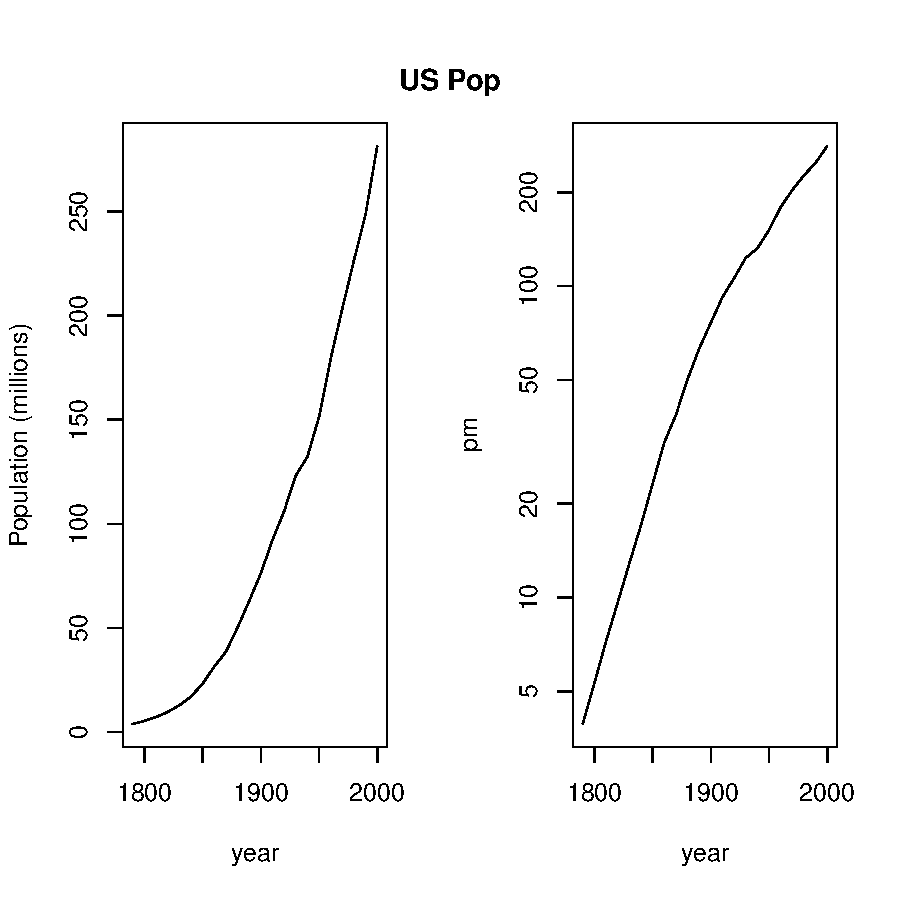
\includegraphics{GRDT-fig1}
\end{center}
\caption{U.S. Population}
\label{fig:one}
\end{figure}
\section*{Growth Rates}
What was the growth rate in the last intercensal period? Let us list the population counts for the last two censuses:
\begin{Schunk}
\begin{Sinput}
> uspop[21:22,]
\end{Sinput}
\begin{Soutput}
   year       pop
21 1990 248709873
22 2000 281421906
\end{Soutput}
\begin{Sinput}
> pop[22]/pop[21] -1
\end{Sinput}
\begin{Soutput}
[1] 0.1315269
\end{Soutput}
\end{Schunk}
So it grew 13.2\% in ten years. You'd think this is 1.32\% per year but that is only approximate because it forgets compounding the growth over the ten years.  If we compound k times per year a rate r we obtain Solving for r gives 
\[
r = k[(P2000/P1990)^{(1/10k)}-1]
\]
Here's the rate we obtain using different values of k
\begin{Schunk}
\begin{Sinput}
> ratio<-pop[22]/pop[21]
> k<-c(1,2,4,6,12,52,365)
> r= k*(ratio^(1/(10*k))-1)
> print(cbind(k,r))
\end{Sinput}
\begin{Soutput}
       k          r
[1,]   1 0.01243345
[2,]   2 0.01239505
[3,]   4 0.01237590
[4,]   6 0.01236953
[5,]  12 0.01236316
[6,]  52 0.01235826
[7,] 365 0.01235700
\end{Soutput}
\end{Schunk}
here 1 means annual, 12 means monthly, and 365 means daily. We could continue compounding every minute, or every second, but you can see that our calculation is approaching a limit. From elementary calculus we know that as k -> infinity our equation becomes P2000=P1990 exp(10r), and solving for r gives log(P2000/P1990)/10, so the limiting value is

\begin{Schunk}
\begin{Sinput}
> log(ratio)/10
\end{Sinput}
\begin{Soutput}
[1] 0.01235679
\end{Soutput}
\end{Schunk}
This, of course, is the mean annualized rate of growth. Note that we got the correct value rounded to five decimal places by the time we compounded monthly.

\section*{Growing more slowly}

We can now compute the growth rate for the entire story of the U.S. We treat all censuses as ten years apart, although this is not exactly true over time they have moved from August to June, and then April xcept for 1920, which was done in Januaryf you want to do a more precise calculation the dates are in the reference given at the top.
\begin{Schunk}
\begin{Sinput}
> growthrate<-c(NA, log(pop[-1]/pop[-22])/10)
\end{Sinput}
\end{Schunk}
Note the use of NA to refer to the first value of population. This generates a missing value for the very first row. Now we plot the rates over time. Because the rate pertains to the period between two censuses it makes more sense to plot it against the mid-point of the dates, which shifts the plot to the right 5 years.
\begin{Schunk}
\begin{Sinput}
> midyear<-c(NA,(year[-1]+year[-22])/2)
\end{Sinput}
\end{Schunk}
The graph is shown in the figure~\ref{fig:dt}, when we combine it with a plot of doubling time. We see that the growth rate declined steadily to reach a minumum in the 1930s, and has since hovered around the 0.9 to 1.7 percent range.

\section*{Doubling Time}
At an instantaneous growth rate r, the doubling time is log(2)/r
\begin{Schunk}
\begin{Sinput}
> doub<-c(NA,log(2)/growthrate[-1])
> par(mfrow=c(1,2))
> plot(midyear,growthrate,type="l", main="Growth Rate")
> plot(midyear,doub, type="l",main="Doubling Time")
> title(main="US 1790-2000\n", outer = T,line=-3)
\end{Sinput}
\end{Schunk}
\begin{figure}[!h]
\begin{center}
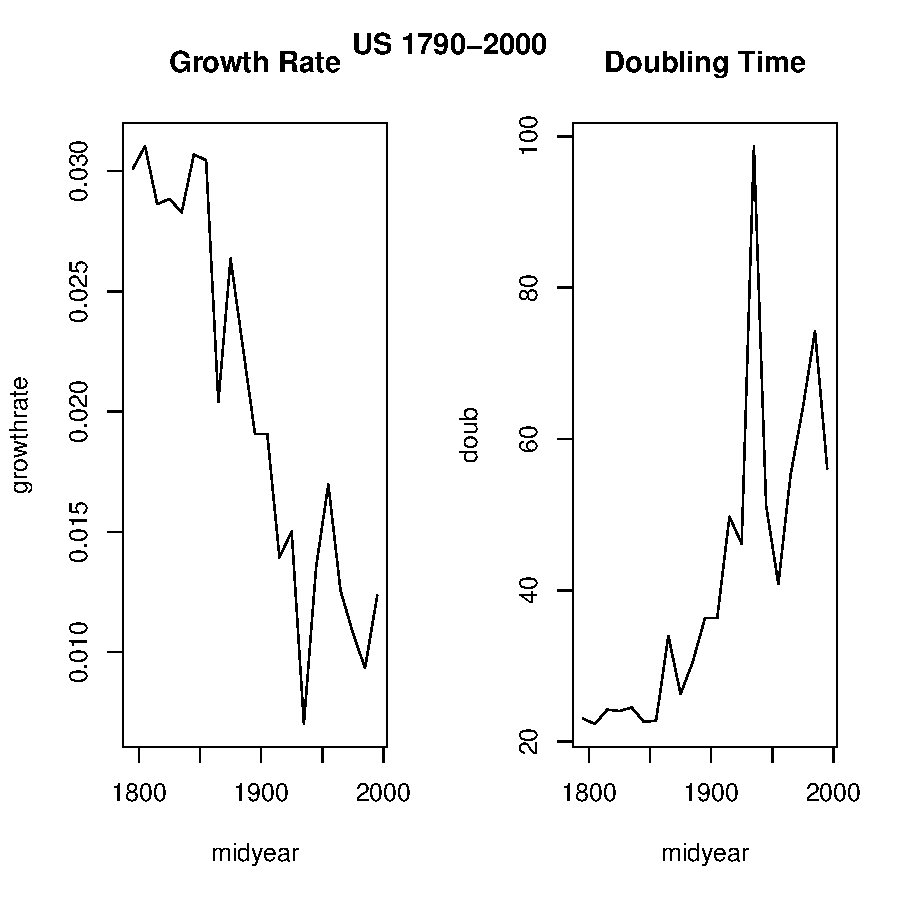
\includegraphics{GRDT-fig2}
\end{center}
\caption{U.S. Population 1790:2000}
\label{fig:dt}
\end{figure}

So the U.S. population was doubling every 22-24 years in the first half of the 19th century, but now it takes 56 years to double.

\end{document}
